%!TEX program = xelatex
%%%%%%%%%%%%%%%%%%%%%%%%%%%%%%%%%%%%%%%%%%%%%%%%%%%%%%%%%%%%%%%%%%%%%%%%%%%%%%%%%
%
% This is a very basic template for mathematical presentations using LaTeX and beamer, aimed at University of Edinburgh students on the Honours Analysis course 2017-2018, for their "Skills" presentations.
%
% This template is just to get you started and to see what the possibilities are.  There is no required format, and you are free to use, discard, edit as much as you like.  I've put in some mathematical content to demonstrate the very basics of LaTeX.  Clearly, you will need to change this.
%
% Except for a few structural comments, I don't comment on the LaTeX itself.  If you have used it before, most of what you know should apply as usual.  If you have not, have a look at the source code, the output, and experiment with editing the code and see what happens.  Most LaTeX code is pretty intuitive, e.g. the command to produce an alpha is \alpha, the command for an integral sign is \int, etc.  You can learn an awful lot by guesswork, trial and error, and google.  
%
% The percent signs "%" are comment signs, and instruct LaTeX to ignore everything following the sign on the same line.  They can be used to comment on the code.
%
%%%%%%%%%%%%%%%%%%%%%%%%%%%%%%%%%%%%%%%%%%%%%%%%%%%%%%%%%%%%%%%%%%%%%%%%%%%%%%%%
%
% The following lines are the preamble.  They help LaTeX set-up the document, but do not print anything yet.

\documentclass{ctexbeamer}		% This tells LaTeX the document will be a "beamer" presentation

\usetheme{Madrid}		% Sets basic formatting.  Lots of options, google "beamer themes"

\usepackage{tikz}
\usepackage[colorlinks,linkcolor=blue]{hyperref}
%%% logo
\pgfdeclareimage[height=0.8cm]{logo}{./logo.png}
\logo{\pgfuseimage{logo}}
%\logo{\vspace*{-0.3cm}\pgfuseimage{logo}}


\usecolortheme{dolphin}	% Sets the colour scheme.  Lots of options, google "beamer color themes"

%\setbeamertemplate{navigation symbols}{}
% Manually changes one piece of formatting.  See what the difference is by commenting this line out.

\date{}	% Insert the date of your presentation. \today gives an unsurprising automatic date.

\title[String]{Manacher, PAM}	% Insert your title.  Depending on the theme you choose above, a "short title" might be useful, as it will appear on the footer of each slide.

\author[calabash\_boy]{calabash\_boy} % Insert your name

\date{\today}

\newcommand{\redP}{{\color{red}\#}}

\begin{document} 	% Let's begin

% Presentations come in slide frames.  You have to tell LaTeX when to start a frame, and when to end the frame.  The most common error beginners make with beamer is forgetting the \end{frame} command.	

\begin{frame}	

\titlepage	% Prints a title page populated with the information given in the preamble
	
\end{frame}		

\begin{frame}{回文串}

\begin{block}{定义}

\textbf{反转串R(S)}:一个字符串$S = S[1]S[2]\cdots S[n]$,其反串为$R(S) = S[n]S[n-1]\cdots S[1]$。

\textbf{回文串}:满足$S = R(S)$的串为回文串。

\pause

\textbf{回文中心}:

\begin{enumerate}
    \item 奇(长度)回文串,回文中心为$S[\frac{n+1}{2}]$,如$ab{\color{red}c}ba$
    \item 偶(长度)回文串,回文中心为$S[\frac{n}{2}]$与$S[\frac{n}{2} + 1]$中间,如$abc{\color{red}{|}}cba$。
\end{enumerate}

\pause

\textbf{回文半径L}:回文中心到回文串的左右端点的距离相等,此距离称为回文半径。

如$ab{\color{red}{c}}ba$半径为3,$abcd{\color{red}|}dcba$半径为4。

\pause

常用二元组\textbf{<回文中心,回文半径>}来表示一个回文子串
\end{block}
    
\end{frame}

\begin{frame}{回文串}

\begin{block}{性质}

\textbf{长度与半径的关系}:
\begin{enumerate}
    \item 奇回文串:$|S| = 2L - 1$
    \item 偶回文串:$|S| = 2L$
\end{enumerate}

\pause

\textbf{回文半径的二分性}:回文半径-1等价于同时删掉回文串的首尾字母,依然是回文串。

\pause

\textbf{回文串和Border}:对于回文串$S$,回文前(后)缀{\color{red}等价于}Border

\end{block}    
    
\end{frame}

\begin{frame}{求回文半径}
    
\begin{block}{问题背景}
给出一个字符串$S$,求每个回文中心的回文半径。包括一个字母作为中心以及两个字母中间的位置作为中心。
\end{block}    

\pause

\begin{block}{不动脑子的做法}
利用回文半径的二分性质,预处理$S$和$R(S)$的Hash,然后利用二分+Hash求每个中心的回文半径。复杂度$O(n\log n)$
\end{block}
\end{frame}

\begin{frame}{Manacher}
\begin{block}{前期处理}
为了将偶回文串的处理方式与奇回文串统一起来,将$S$的每两个字母中间,以及开头结尾插入$\redP$。

例如$S = bccbeb$,预处理后变为$S^{\redP} = \redP b\redP c\redP c\redP b\redP e\redP b\redP$。

\pause

因此所有回文串都变成奇数长度,且首尾一定是$\redP$。例如
\begin{enumerate}
    \item 原始偶回文串:$bccb^{\redP} = \redP b\redP c\redP c\redP b\redP$,长度为9,回文中心是$\redP$
    \item 原始奇回文串:$beb^{\redP} = \redP b\redP e\redP b\redP$,长度为7,回文中心是$e$
\end{enumerate}

\pause

同时,所有极长回文子串长度一定为奇数:因为极长回文子串一定以$\redP$开头结尾。

\pause

容易发现:$|S^{\redP}| = 2|S| + 1$,\hspace{2pt} 以及$|S| = \frac{|S^{\redP}| - 1}{2} = \lfloor\frac{|S^{\redP}|}{2}\rfloor$。容易验证此关系对回文半径依然适用。

\end{block}
    
\end{frame}


\begin{frame}{Manacher}

\begin{block}{定义}
$Len[i]$表示以$i$为回文中心的最大回文半径。

\textbf{最右回文串P}:所有已求得的回文串中,右端点最靠右的一个。

\end{block}

\pause

\begin{block}{算法流程}

从左到右求每个位置的回文半径,同时维护最右回文串$S[L,R]$及其回文中心$p$。

\pause

设当前$1,2,\cdots, i-1$位置的$Len$已经求出,当前需要求$Len[i]$,根据$i$与$[L,R]$的关系,总共分三类情况讨论:

\end{block}
\end{frame}

\begin{frame}{Manacher}

\begin{block}{算法流程}
{\color{red}1、$i > R$:}

\begin{figure}[h]
    \centering

\begin{tikzpicture}

\fill[blue, very thick] (0,0) rectangle (1, 0.5);
\fill[green, very thick] (1,0) rectangle (8.5, 0.5);
\node (shape) at (4.75, 0.25) [draw] {p};
\node (shape) at (1.25, 0.25) [draw] {L};
\node (shape) at (8.25, 0.25) [draw] {R};
\draw [black, very thick] (1,0) rectangle (8.5, 0.5);

\fill[gray, very thick] (8.5, 0) rectangle (11, 0.5);

\node (shape) at (8.7, 0.25) [draw] {I};

\end{tikzpicture}
 
\end{figure} 

以$i$为回文中心,向左向右{\color{red}暴力}拓展,求得回文半径$Len[i]$,同时最右回文串会变为:

$p = i$

$L = i - Len[i] + 1$

$R = i + Len[i] - 1$


\pause

\begin{figure}[h]
    \centering
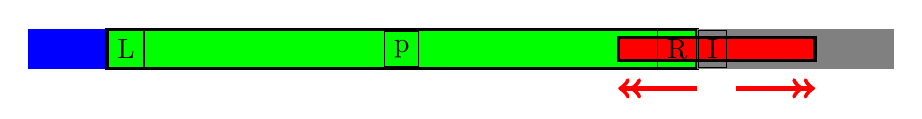
\begin{tikzpicture}

\fill[blue, very thick] (0,0) rectangle (1, 0.5);
\fill[green, very thick] (1,0) rectangle (8.5, 0.5);

\draw [black, very thick] (1,0) rectangle (8.5, 0.5);

\fill[gray, very thick] (8.5, 0) rectangle (11, 0.5);


\fill [red, very thick] (7.5, 0.1) rectangle (10, 0.4);
\draw [black, very thick] (7.5, 0.1) rectangle (10, 0.4);

\draw [->>, red,ultra thick] (8.5, -0.25) -- (7.5, -0.25);

\draw [->>, red, ultra thick] (9, -0.25) -- (10, -0.25);
\node (shape) at (4.75, 0.25) [draw] {p};
\node (shape) at (1.25, 0.25) [draw] {L};
\node (shape) at (8.25, 0.25) [draw] {R};
\node (shape) at (8.7, 0.25) [draw] {I};


\end{tikzpicture}
 
\end{figure} 

\end{block}
    
\end{frame}

\begin{frame}{Manacher}

\begin{block}{算法流程}
{\color{red}2、$i \leq R$:}

\begin{figure}[h]
    \centering

\begin{tikzpicture}

\fill[blue, very thick] (0,0) rectangle (1, 0.5);
\fill[green, very thick] (1,0) rectangle (8.5, 0.5);
\node (shape) at (4.75, 0.25) [draw] {p};
\node (shape) at (1.25, 0.25) [draw] {L};
\node (shape) at (8.25, 0.25) [draw] {R};
\draw [black, very thick] (1,0) rectangle (8.5, 0.5);

\fill[gray, very thick] (8.5, 0) rectangle (11, 0.5);

\node (i) at (6.75, 0.25) [draw] {I};

\end{tikzpicture}
 
\end{figure} 

由于回文串的对称性:最右回文串P的左半和右半是对称的。找到$i$关于$p$的对称位置$j = 2p - i$。
\begin{figure}[h]
    \centering
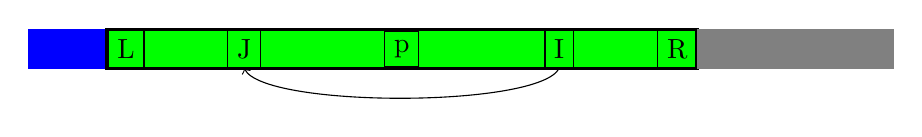
\begin{tikzpicture}

\fill[blue, very thick] (0,0) rectangle (1, 0.5);
\fill[green, very thick] (1,0) rectangle (8.5, 0.5);
\node (shape) at (4.75, 0.25) [draw] {p};
\node (shape) at (1.25, 0.25) [draw] {L};
\node (shape) at (8.25, 0.25) [draw] {R};
\draw [black, very thick] (1,0) rectangle (8.5, 0.5);

\fill[gray, very thick] (8.5, 0) rectangle (11, 0.5);

\node (i) at (6.75, 0.25) [draw] {I};

\node (j) at (2.75, 0.25) [draw] {J};

\draw [->] (i.south) .. controls (6.5, -0.5) and (3, -0.5) .. (j.south);

\end{tikzpicture}
 
\end{figure} 

由于$Len[j]$是已经求得的,根据最右回文串的对称性,$Len[i]$可以直接继承$Len[j]$在最右回文串范围内的部分,根据$Len[j]$是否超出了最右回文串的范围,继续讨论两种情况。

\end{block}
    
\end{frame}

\begin{frame}{Manacher}

\begin{block}{算法流程}

{\color{red}2.1、$j - Len[j] + 1 > L$}


\begin{figure}[h]
    \centering

\begin{tikzpicture}

\fill[blue, very thick] (0,0) rectangle (1, 0.5);
\fill[green, very thick] (1,0) rectangle (8.5, 0.5);
\node (shape) at (4.75, 0.25) [draw] {p};
\node (shape) at (1.25, 0.25) [draw] {L};
\node (shape) at (8.25, 0.25) [draw] {R};
\draw [black, very thick] (1,0) rectangle (8.5, 0.5);

\fill[gray, very thick] (8.5, 0) rectangle (11, 0.5);

\fill [yellow, very thick] (1.75, 0.1) rectangle (3.75, 0.4);
\draw [black, very thick] (1.75, 0.1) rectangle (3.75, 0.4);

\node (i) at (6.75, 0.25) [draw] {I};

\node (j) at (2.75, 0.25) [draw] {J};


\end{tikzpicture}
\end{figure}

由于$Len[j]$没有超出最右回文串的表示范围,由对称性,可以确定$Len[i] = Len[j]$,且不能够再拓展。

\pause

\begin{figure}[h]
    \centering
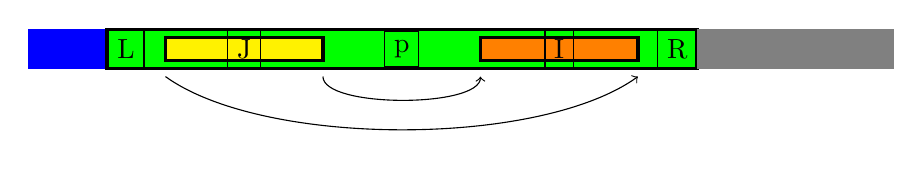
\begin{tikzpicture}

\fill[blue, very thick] (0,0) rectangle (1, 0.5);
\fill[green, very thick] (1,0) rectangle (8.5, 0.5);
\node (shape) at (4.75, 0.25) [draw] {p};
\node (shape) at (1.25, 0.25) [draw] {L};
\node (shape) at (8.25, 0.25) [draw] {R};
\draw [black, very thick] (1,0) rectangle (8.5, 0.5);

\fill[gray, very thick] (8.5, 0) rectangle (11, 0.5);

\fill [yellow, very thick] (1.75, 0.1) rectangle (3.75, 0.4);
\draw [black, very thick] (1.75, 0.1) rectangle (3.75, 0.4);

\fill [orange, very thick] (5.75, 0.1) rectangle (7.75, 0.4);
\draw [black, very thick] (5.75, 0.1) rectangle (7.75, 0.4);

\node (i) at (6.75, 0.25) [draw] {I};

\node (j) at (2.75, 0.25) [draw] {J};

\draw [->] (1.75, -0.1) .. controls (3, -1) and (6.5, -1) .. (7.75, -0.1);

\draw [->] (3.75, -0.1) .. controls (3.75, -0.5) and (5.75, -0.5) .. (5.75, -0.1);

\end{tikzpicture}
 
\end{figure} 

此时,最右回文串没有发生变化。

\end{block}

\end{frame}


\begin{frame}{Manacher}
    
\begin{block}{算法流程}
{\color{red}2.2、$j-Len[j]+1 \leq L$}

\begin{figure}[h]
    \centering

\begin{tikzpicture}

\fill[blue, very thick] (0,0) rectangle (1, 0.5);
\fill[green, very thick] (1,0) rectangle (8.5, 0.5);

\draw [black, very thick] (1,0) rectangle (8.5, 0.5);

\fill[gray, very thick] (8.5, 0) rectangle (11, 0.5);

\draw [black, very thick] (0.75, 0.1) rectangle (4.25, 0.4);
\fill [yellow, very thick] (0.75, 0.1) rectangle (4.25, 0.4);

\node (shape) at (4.75, 0.25) [draw] {p};
\node (shape) at (1.25, 0.25) [draw] {L};
\node (shape) at (8.25, 0.25) [draw] {R};

\node (i) at (7, 0.25) [draw] {I};

\node (j) at (2.5, 0.25) [draw] {J};
\end{tikzpicture}
\end{figure}


由于$Len[j]$超出了最右回文串的范围,且灰色部分的值未知,因此$Len[i]$至多只能继承到最右回文串范围内的$Len[j]$,即$Len[i] <- j - L + 1$

\pause

\begin{figure}[h]
    \centering
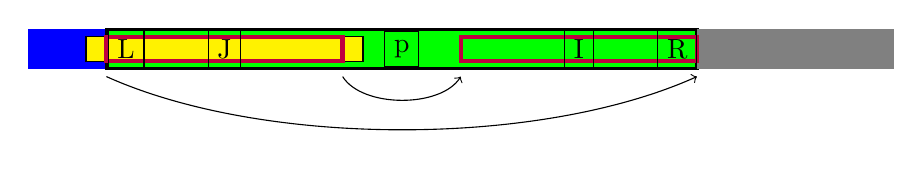
\begin{tikzpicture}

\fill[blue, very thick] (0,0) rectangle (1, 0.5);
\fill[green, very thick] (1,0) rectangle (8.5, 0.5);

\draw [black, very thick] (1,0) rectangle (8.5, 0.5);

\fill[gray, very thick] (8.5, 0) rectangle (11, 0.5);

\draw [black, very thick] (0.75, 0.1) rectangle (4.25, 0.4);
\fill [yellow, very thick] (0.75, 0.1) rectangle (4.25, 0.4);

\draw [purple, ultra thick] (1, 0.1) rectangle (4, 0.4);
\draw [purple, ultra thick] (5.5, 0.1) rectangle (8.5, 0.4);
\node (shape) at (4.75, 0.25) [draw] {p};
\node (shape) at (1.25, 0.25) [draw] {L};
\node (shape) at (8.25, 0.25) [draw] {R};

\node (i) at (7, 0.25) [draw] {I};

\node (j) at (2.5, 0.25) [draw] {J};

\draw [->] (4, -0.1) .. controls (4.25, -0.5) and (5.25, -0.5) .. (5.5, -0.1);
\draw [->] (1, -0.1) .. controls (3, -1) and (6.5, -1) .. (8.5, -0.1);

\end{tikzpicture}
\end{figure}

之后由于灰色部分的值未知,因此需要继续向左向右{\color{red}暴力}拓展。

\pause

\begin{figure}[h]
    \centering
\begin{tikzpicture}

\fill[blue, very thick] (0,0) rectangle (8.5, 0.5);


\fill[gray, very thick] (8.5, 0) rectangle (11, 0.5);

\fill [orange, ultra thick] (5.5, 0.1) rectangle (8.5, 0.4);

\fill [red, ultra thick] (3.5, 0.1) rectangle (5.5, 0.4);
\fill [red, ultra, thick] (8.5, 0.1) rectangle (10.5, 0.4);
\draw [black, ultra thick] (3.5, 0.1) rectangle (10.5, 0.4);
\node (i) at (7, 0.25) [draw] {I};

\draw [->>, red,ultra thick] (5.5, -0.25) -- (3.5, -0.25);

\draw [->>, red, ultra thick] (8.5, -0.25) -- (10.5, -0.25);

\end{tikzpicture}
\end{figure}

最右回文串会更新为i。
\end{block}
\end{frame}


\begin{frame}{Manacher}

\begin{block}{复杂度分析}

每次暴力匹配一定伴随着最右回文串右端点$R$的右移。因此复杂度为线性。

\end{block}

\pause

\begin{block}{用法}
1. 求每个回文中心的回文半径

2. 求本质不同回文串:在Manacher中,新的回文串一定出现在使得最右串右移的时候。因此本质不同回文串至多$n$个,把所有更新最右回文串去重即得到本质不同回文串。
\end{block}
    
\end{frame}

\begin{frame}{例题1}
    
\begin{block}{\href{https://ac.nowcoder.com/acm/contest/5633/F}{例题1}}
给出一个字符串$S$,和$Q$次询问,每次询问$S[L,R]$有多少个回文子串。
\end{block}

\pause
\begin{block}{题解}
从询问入手,由于回文串天生的对称性,因此可以把问题分成左右两半来思考:

\pause

如果回文串的中心在询问区间的左半边,那么左端点将称为回文半径长度的唯一限制,中心在右半边同理。

\pause

利用Manacher预处理回文半径,之后问题将变为二维数点。
\end{block}

\end{frame}

\begin{frame}{例题2}
    
\begin{block}{\href{https://www.luogu.com.cn/problem/P1659}{某谷P1659}}
给出一个字符串$S$,$|S| \leq 1000, 000$。求前$K$大的回文子串长度乘积。

$K \leq 1000, 000, 000$。
\end{block}

\pause

\begin{block}{题解}
首先用Manacher处理每个位置的回文半径,于是每个位置代表了一系列的回文串:

长度分别为$X, X -2, X -4, \cdots, 0/1$。

从大到小扫描,边合并边计算乘积即可。

\end{block}
\end{frame}


\begin{frame}{例题3}

\begin{block}{\href{https://www.luogu.com.cn/problem/P4555}{某谷P4555}}
给出一个字符串$S$,求最长的双回文子串。

回文双子串$T$定义为:可以从一个位置切开,使得前缀和后缀都是回文串。

$|S| \leq 100,000$.
\end{block}
\pause

\begin{block}{题解}
可以枚举拼接点,然后分别最大化以该点为左端点和右端点的回文串长度。

即等价于最大化 左侧回文串和右侧回文串的回文半径。

\pause

利用Manacher求出回文半径之后,配合线段树等数据结构进行区间更新和查询即可。
\end{block}
    
\end{frame}

\begin{frame}{例题3}

\begin{block}{\href{https://www.luogu.com.cn/problem/P3501}{某谷P3501}}
给出一个01串$S$,求最长的反对称子串。

反对称串$T$定义为:将$R(T)$逐位取反之后等于原串$T$,则$T$是一个反对称串,例如$010101$。

$|S| \leq 500, 000$
\end{block}

\pause

\begin{block}{题解}
在新的相等运算意义下进行Manacher即可。
\end{block}
    
\end{frame}

\begin{frame}{例题4}
    
\begin{block}{\href{https://www.luogu.com.cn/problem/P4287}{某谷 P4287}}

给出一个字符串$S$,求最长的双倍回文子串。若一个串能表示成$T\hspace{2pt}R(T)T\hspace{2pt}R(T)$的形式,则称为一个双倍回文串,例如$ab{\color{red}ba}ab{\color{red}ba}$。

$|S| \leq 500, 000$.

\end{block}

\pause

\begin{block}{题解}

由于本质不同回文串只有n个,因此逐一检查是否是双倍回文即可。
\pause
由于新的回文串一定发生于更新最右回文串的时候,所以在发生暴力拓展的时候,顺便检查即可。

\end{block}

\end{frame}

\begin{frame}{PAM}

\begin{block}{定义}
Palindrome Automaton(回文自动机,回文树)是一种能够识别所有回文子串的数据结构,结构十分类似于之前讲的ACAM。


\pause

\begin{enumerate}
    \item 节点:节点数至多$N$个,每个节点代表了一种回文串。用$S(u)$表示节点$u$代表的回文串。$len[u] = |S(u)|$

    \pause

    \item 后继边:每个后继边上有一个字母。用$trans(u,ch) = v$表示$u$节点有后继边$ch$指向$v$节点。 则有$S(v) = \textbf{ch} S(u) \textbf{ch}$,以及$len[v] = len[u] + 2$
    
    \pause
    
    \item 失配边:每个节点都有一个失配边,用$fail[u] = v$表示$u$节点的失配边指向了$v$节点。 则有$S(v)$是$S(u)$的最大Border,即最长回文后缀。

\end{enumerate}
\end{block}
\end{frame}

\begin{frame}{PAM}

\begin{block}{PAM的构造}

PAM在构造时,实际上就是求每个前缀的最长回文后缀,方法是枚举前一个位置的回文后缀,即fail链。
\begin{figure}
    \centering
    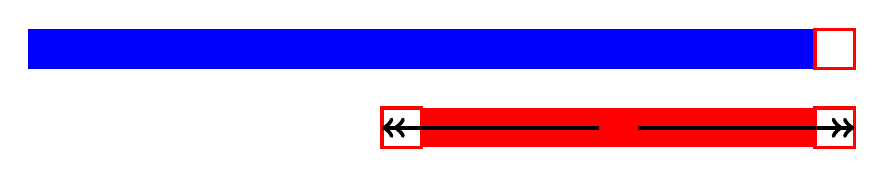
\begin{tikzpicture}
    \fill[blue] (0,0) rectangle (10, 0.5);
    \draw[red, very thick] (10, 0) rectangle (10.5, 0.5);
    
    \draw[red, very thick] (10, -1) rectangle (10.5, -0.5);
    \fill[red] (5, -1) rectangle (10, -0.5);
    \draw[red, very thick] (4.5, -1) rectangle (5, -0.5);
    
    \draw [black, ->>, ultra thick] (7.25, -0.75) -- (4.5, -0.75);
    \draw [black, ->>, ultra thick] (7.75, -0.75) -- (10.5, -0.75);
    \end{tikzpicture}
\end{figure}
    
\end{block}    
\end{frame}

\begin{frame}{PAM}

\begin{block}{PAM的构造}

PAM在构造时,实际上就是求每个前缀的最长回文后缀,方法是枚举前一个位置的回文后缀,即fail链。
\begin{figure}
    \centering
    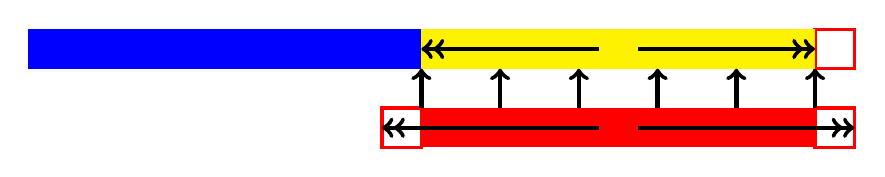
\begin{tikzpicture}
    \fill[blue] (0,0) rectangle (10, 0.5);
    \draw[red, very thick] (10, 0) rectangle (10.5, 0.5);
    
    \draw[red, very thick] (10, -1) rectangle (10.5, -0.5);
    \fill[red] (5, -1) rectangle (10, -0.5);
    \draw[red, very thick] (4.5, -1) rectangle (5, -0.5);
    
    \draw [black, ->>, ultra thick] (7.25, -0.75) -- (4.5, -0.75);
    \draw [black, ->>, ultra thick] (7.75, -0.75) -- (10.5, -0.75);
    
    
    \fill[yellow] (5, 0) rectangle (10, 0.5);
    
    \draw[black, ->>, ultra thick] (7.25, 0.25) -- (5, 0.25);
    \draw[black, ->>, ultra thick] (7.75, 0.25) -- (10, 0.25);
    
    \draw[black, ->, ultra thick] (5, -0.5) -- (5, 0);
    \draw[black, ->, ultra thick] (10, -0.5) -- (10, 0);
    \draw[black, ->, ultra thick] (7, -0.5) -- (7, 0);
    \draw[black, ->, ultra thick] (8, -0.5) -- (8, 0);
    \draw[black, ->, ultra thick] (6, -0.5) -- (6, 0);
    \draw[black, ->, ultra thick] (9, -0.5) -- (9, 0);
    \end{tikzpicture}
\end{figure}



\pause

PAM特殊之处在于:对于奇回文串和偶回文串需要有两个根节点。

由于长度为2的回文串是偶根的后继节点,长度为1的回文串是奇根的后继节点。

因此偶根长度应设为0,奇根应该设为-1。

\pause

方便起见,可以令偶根的失配边指向奇根,奇根的失配边指向偶根。

\end{block}    
    
\end{frame}

\begin{frame}{PAM}
$S = abacabbaca$.

1表示奇根,0表示偶根。方括号表示长度。Last指针指向偶根0.

\begin{figure}
    \centering
\begin{tikzpicture}[greennode/.style={circle, draw=green!60, fill=green!5, very thick, minimum size=7mm},
blacknode/.style={circle, draw=black!60, fill=grey!5, very thick, minimum size=7mm},
redline/.style={->, dashed, color = red, line width = 2pt},
blueline/.style={->, dashed, color = blue, line width = 1.5pt}]

\node[greennode] (root1) at (0,0) {1\color{red}[-1]};
\node[greennode] (root2) at (-2, 0) {0\color{red}[0]};

\draw[redline] (root2.north east) ..controls (-1, 0.5) .. (root1.north west);
\draw[redline] (root1.south west) .. controls (-1, -0.5) .. (root2.south east);

\node[square, draw] (Last) at (-5, 0) {Last};
\draw[->] (Last.east) -- (root2.west);

\end{tikzpicture}
\end{figure}
\end{frame}

\begin{frame}{PAM}
$S = {\color{red}a}bacabbaca$.

\begin{figure}
    \centering
\begin{tikzpicture}[greennode/.style={circle, draw=green!60, fill=green!5, very thick, minimum size=7mm},
blacknode/.style={circle, draw=black!60, fill=grey!5, very thick, minimum size=7mm},
redline/.style={->, dashed, color = red, line width = 2pt},
blueline/.style={->, dashed, color = blue, line width = 1.5pt}]

\node[blacknode] (root1) at (0,0) {1\color{red}[-1]};
\node[blacknode] (root2) at (-2, 0) {0\color{red}[0]};

\draw[blueline] (root2.north east) ..controls (-1, 0.5) .. (root1.north west);
\draw[blueline] (root1.south west) .. controls (-1, -0.5) .. (root2.south east);

\node[greennode] (a) at (0, -2) {2\color{red}[1]};
\draw[->] (root1.south) -- (a.north);
\node at (0.2, -1) {$a$};
\draw[redline] (a.north west) .. controls (-1.25, -1.25) .. (root2.south east);

\node[square, draw] (Last) at (4, -2) {Last};
\draw[->] (Last.west) -- (a.east);

\end{tikzpicture}
\end{figure}
\end{frame}

\begin{frame}{PAM}
$S = a{\color{red}b}acabbaca$.

\begin{figure}
    \centering
\begin{tikzpicture}[greennode/.style={circle, draw=green!60, fill=green!5, very thick, minimum size=7mm},
blacknode/.style={circle, draw=black!60, fill=grey!5, very thick, minimum size=7mm},
redline/.style={->, dashed, color = red, line width = 2pt},
blueline/.style={->, dashed, color = blue, line width = 1.5pt}]

\node[blacknode] (root1) at (0,0) {1\color{red}[-1]};
\node[blacknode] (root2) at (-2, 0) {0\color{red}[0]};

\draw[blueline] (root2.north east) ..controls (-1, 0.5) .. (root1.north west);
\draw[blueline] (root1.south west) .. controls (-1, -0.5) .. (root2.south east);

\node[blacknode] (a) at (0, -2) {2\color{red}[1]};
\draw[->] (root1.south) -- (a.north);
\node at (0.2, -1) {$a$};
\draw[blueline] (a.north west) .. controls (-1.25, -1.25) .. (root2.south east);

\node[greennode] (b) at (2, -2) {3\color{red}[1]};
\draw[->] (root1.south east) -- (b.north);
\node at (1.2, -1) {$b$};
\draw[redline] (b.north west) .. controls (0, -1.25) and (-1.25, -1.25).. (root2.south east);


\node[square, draw] (Last) at (5, -2) {Last};
\draw[->] (Last.west) -- (b.east);

\end{tikzpicture}
\end{figure}
\end{frame}

\begin{frame}{PAM}
$S = {\color{red}aba}cabbaca$.

\begin{figure}
    \centering
\begin{tikzpicture}[greennode/.style={circle, draw=green!60, fill=green!5, very thick, minimum size=7mm},
blacknode/.style={circle, draw=black!60, fill=grey!5, very thick, minimum size=7mm},
redline/.style={->, dashed, color = red, line width = 2pt},
blueline/.style={->, dashed, color = blue, line width = 1.5pt}]

\node[blacknode] (root1) at (0,0) {1\color{red}[-1]};
\node[blacknode] (root2) at (-2, 0) {0\color{red}[0]};

\draw[blueline] (root2.north east) ..controls (-1, 0.5) .. (root1.north west);
\draw[blueline] (root1.south west) .. controls (-1, -0.5) .. (root2.south east);

\node[blacknode] (a) at (0, -2) {2\color{red}[1]};
\draw[->] (root1.south) -- (a.north);
\node at (0.2, -1) {$a$};
\draw[blueline] (a.north west) .. controls (-1.25, -1.25) .. (root2.south east);

\node[blacknode] (b) at (2, -2) {3\color{red}[1]};
\draw[->] (root1.south east) -- (b.north);
\node at (1.25, -0.95) {$b$};
\draw[blueline] (b.north west) .. controls (0, -1.25) and (-1.25, -1.25).. (root2.south east);

\node[greennode] (aba) at (2, -4) {4\color{red}[3]};
\draw[->] (b.south) -- (aba.north);
\node at (2.2, -3) {$a$};
\draw[redline] (aba.north west) .. controls (0.9, -3.1) .. (a.south east);


\node[square, draw] (Last) at (5, -4) {Last};
\draw[->] (Last.west) -- (aba.east);

\end{tikzpicture}
\end{figure}
\end{frame}

\begin{frame}{PAM}
$S = aba{\color{red}c}abbaca$.

\begin{figure}
    \centering
\begin{tikzpicture}[greennode/.style={circle, draw=green!60, fill=green!5, very thick, minimum size=7mm},
blacknode/.style={circle, draw=black!60, fill=grey!5, very thick, minimum size=7mm},
redline/.style={->, dashed, color = red, line width = 2pt},
blueline/.style={->, dashed, color = blue, line width = 1.5pt}]

\node[blacknode] (root1) at (0,0) {1\color{red}[-1]};
\node[blacknode] (root2) at (-2, 0) {0\color{red}[0]};

\draw[blueline] (root2.north east) ..controls (-1, 0.5) .. (root1.north west);
\draw[blueline] (root1.south west) .. controls (-1, -0.5) .. (root2.south east);

\node[blacknode] (a) at (0, -2) {2\color{red}[1]};
\draw[->] (root1.south) -- (a.north);
\node at (0.2, -1) {$a$};
\draw[blueline] (a.north west) .. controls (-1.25, -1.25) .. (root2.south east);

\node[blacknode] (b) at (2, -2) {3\color{red}[1]};
\draw[->] (root1.south east) -- (b.north);
\node at (1.25, -0.95) {$b$};
\draw[blueline] (b.north west) .. controls (0, -1.25) and (-1.25, -1.25).. (root2.south east);

\node[blacknode] (aba) at (2, -4) {4\color{red}[3]};
\draw[->] (b.south) -- (aba.north);
\node at (2.2, -3) {$a$};
\draw[blueline] (aba.north west) .. controls (0.9, -3.1) .. (a.south east);

\node[greennode] (c) at (4, -2) {5\color{red}[1]};
\draw[->] (root1.south east) -- (c.north);
\node at (2.1, -0.9) {$c$};
\draw[redline] (c.north west) .. controls (0, -1.25) and (-1.25, -1.25) .. (root2.south east);

\node[square, draw] (Last) at (7, -2) {Last};
\draw[->] (Last.west) -- (c.east);

\end{tikzpicture}
\end{figure}
\end{frame}

\begin{frame}{PAM}
$S = ab{\color{red}aca}bbaca$.

\begin{figure}
    \centering
\begin{tikzpicture}[greennode/.style={circle, draw=green!60, fill=green!5, very thick, minimum size=7mm},
blacknode/.style={circle, draw=black!60, fill=grey!5, very thick, minimum size=7mm},
redline/.style={->, dashed, color = red, line width = 2pt},
blueline/.style={->, dashed, color = blue, line width = 1.5pt}]

\node[blacknode] (root1) at (0,0) {1\color{red}[-1]};
\node[blacknode] (root2) at (-2, 0) {0\color{red}[0]};

\draw[blueline] (root2.north east) ..controls (-1, 0.5) .. (root1.north west);
\draw[blueline] (root1.south west) .. controls (-1, -0.5) .. (root2.south east);

\node[blacknode] (a) at (0, -2) {2\color{red}[1]};
\draw[->] (root1.south) -- (a.north);
\node at (0.2, -1) {$a$};
\draw[blueline] (a.north west) .. controls (-1.25, -1.25) .. (root2.south east);

\node[blacknode] (b) at (2, -2) {3\color{red}[1]};
\draw[->] (root1.south east) -- (b.north);
\node at (1.25, -0.95) {$b$};
\draw[blueline] (b.north west) .. controls (0, -1.25) and (-1.25, -1.25).. (root2.south east);

\node[blacknode] (aba) at (2, -4) {4\color{red}[3]};
\draw[->] (b.south) -- (aba.north);
\node at (2.2, -3) {$a$};
\draw[blueline] (aba.north west) .. controls (0.9, -3.1) .. (a.south east);

\node[blacknode] (c) at (4, -2) {5\color{red}[1]};
\draw[->] (root1.south east) -- (c.north);
\node at (2.1, -0.9) {$c$};
\draw[blueline] (c.north west) .. controls (0, -1.25) and (-1.25, -1.25) .. (root2.south east);

\node[greennode] (aca) at (4, -4) {6\color{red}[3]};
\draw[->] (c.south) -- (aca.north);
\node at (4.2, -3) {$a$};
\draw[redline] (aca.north west) .. controls (2, -3.2) .. (a.south east);

\node[square, draw] (Last) at (7, -4) {Last};
\draw[->] (Last.west) -- (aca.east);

\end{tikzpicture}
\end{figure}
\end{frame}

\begin{frame}{PAM}
$S = a{\color{red}bacab}baca$.

\begin{figure}
    \centering
\begin{tikzpicture}[greennode/.style={circle, draw=green!60, fill=green!5, very thick, minimum size=7mm},
blacknode/.style={circle, draw=black!60, fill=grey!5, very thick, minimum size=7mm},
redline/.style={->, dashed, color = red, line width = 2pt},
blueline/.style={->, dashed, color = blue, line width = 1.5pt}]

\node[blacknode] (root1) at (0,0) {1\color{red}[-1]};
\node[blacknode] (root2) at (-2, 0) {0\color{red}[0]};

\draw[blueline] (root2.north east) ..controls (-1, 0.5) .. (root1.north west);
\draw[blueline] (root1.south west) .. controls (-1, -0.5) .. (root2.south east);

\node[blacknode] (a) at (0, -2) {2\color{red}[1]};
\draw[->] (root1.south) -- (a.north);
\node at (0.2, -1) {$a$};
\draw[blueline] (a.north west) .. controls (-1.25, -1.25) .. (root2.south east);

\node[blacknode] (b) at (2, -2) {3\color{red}[1]};
\draw[->] (root1.south east) -- (b.north);
\node at (1.25, -0.95) {$b$};
\draw[blueline] (b.north west) .. controls (0, -1.25) and (-1.25, -1.25).. (root2.south east);

\node[blacknode] (aba) at (2, -4) {4\color{red}[3]};
\draw[->] (b.south) -- (aba.north);
\node at (2.2, -3) {$a$};
\draw[blueline] (aba.north west) .. controls (0.9, -3.1) .. (a.south east);

\node[blacknode] (c) at (4, -2) {5\color{red}[1]};
\draw[->] (root1.south east) -- (c.north);
\node at (2.1, -0.9) {$c$};
\draw[blueline] (c.north west) .. controls (0, -1.25) and (-1.25, -1.25) .. (root2.south east);

\node[blacknode] (aca) at (4, -4) {6\color{red}[3]};
\draw[->] (c.south) -- (aca.north);
\node at (4.2, -3) {$a$};
\draw[blueline] (aca.north west) .. controls (2, -3.2) .. (a.south east);

\node[greennode] (bacab) at (4, -6) {7\color{red}[5]};
\draw[->] (aca.south) -- (bacab.north);
\node at (4.2, -5) {$b$};
\draw[redline] (bacab.north west) .. controls (3, -5.1) .. (b.south east);

\node[square, draw] (Last) at (-2, -6) {Last};
\draw[->] (Last.east) -- (bacab.west);

\end{tikzpicture}
\end{figure}
\end{frame}

\begin{frame}{PAM}
$S = abaca{\color{red}bb}aca$.

\begin{figure}
    \centering
\begin{tikzpicture}[greennode/.style={circle, draw=green!60, fill=green!5, very thick, minimum size=7mm},
blacknode/.style={circle, draw=black!60, fill=grey!5, very thick, minimum size=7mm},
redline/.style={->, dashed, color = red, line width = 2pt},
blueline/.style={->, dashed, color = blue, line width = 1.5pt}]

\node[blacknode] (root1) at (0,0) {1\color{red}[-1]};
\node[blacknode] (root2) at (-2, 0) {0\color{red}[0]};

\draw[blueline] (root2.north east) ..controls (-1, 0.5) .. (root1.north west);
\draw[blueline] (root1.south west) .. controls (-1, -0.5) .. (root2.south east);

\node[blacknode] (a) at (0, -2) {2\color{red}[1]};
\draw[->] (root1.south) -- (a.north);
\node at (0.2, -1) {$a$};
\draw[blueline] (a.north west) .. controls (-1.25, -1.25) .. (root2.south east);

\node[blacknode] (b) at (2, -2) {3\color{red}[1]};
\draw[->] (root1.south east) -- (b.north);
\node at (1.25, -0.95) {$b$};
\draw[blueline] (b.north west) .. controls (0, -1.25) and (-1.25, -1.25).. (root2.south east);

\node[blacknode] (aba) at (2, -4) {4\color{red}[3]};
\draw[->] (b.south) -- (aba.north);
\node at (2.2, -3) {$a$};
\draw[blueline] (aba.north west) .. controls (0.9, -3.1) .. (a.south east);

\node[blacknode] (c) at (4, -2) {5\color{red}[1]};
\draw[->] (root1.south east) -- (c.north);
\node at (2.1, -0.9) {$c$};
\draw[blueline] (c.north west) .. controls (0, -1.25) and (-1.25, -1.25) .. (root2.south east);

\node[blacknode] (aca) at (4, -4) {6\color{red}[3]};
\draw[->] (c.south) -- (aca.north);
\node at (4.2, -3) {$a$};
\draw[blueline] (aca.north west) .. controls (2, -3.2) .. (a.south east);

\node[blacknode] (bacab) at (4, -6) {7\color{red}[5]};
\draw[->] (aca.south) -- (bacab.north);
\node at (4.2, -5) {$b$};
\draw[blueline] (bacab.north west) .. controls (3, -5.1) .. (b.south east);

\node[greennode] (bb) at (-2, -2) {8\color{red}[2]};
\draw[->] (root2.south) -- (bb.north);
\node at (-1.8, -1) {$b$};
\draw[redline] (bb.south east) .. controls (0, -3) .. (b.south west);

\node[square, draw] (Last) at (-4, -2) {Last};
\draw[->] (Last.east) -- (bb.west);

\end{tikzpicture}
\end{figure}
\end{frame}

\begin{frame}{PAM}
$S = abacabb{\color{red}a}ca$.

\begin{figure}
    \centering
\begin{tikzpicture}[greennode/.style={circle, draw=green!60, fill=green!5, very thick, minimum size=7mm},
blacknode/.style={circle, draw=black!60, fill=grey!5, very thick, minimum size=7mm},
redline/.style={->, dashed, color = red, line width = 2pt},
blueline/.style={->, dashed, color = blue, line width = 1.5pt}]

\node[blacknode] (root1) at (0,0) {1\color{red}[-1]};
\node[blacknode] (root2) at (-2, 0) {0\color{red}[0]};

\draw[blueline] (root2.north east) ..controls (-1, 0.5) .. (root1.north west);
\draw[blueline] (root1.south west) .. controls (-1, -0.5) .. (root2.south east);

\node[greennode] (a) at (0, -2) {2\color{red}[1]};
\draw[->] (root1.south) -- (a.north);
\node at (0.2, -1) {$a$};
\draw[blueline] (a.north west) .. controls (-1.25, -1.25) .. (root2.south east);

\node[blacknode] (b) at (2, -2) {3\color{red}[1]};
\draw[->] (root1.south east) -- (b.north);
\node at (1.25, -0.95) {$b$};
\draw[blueline] (b.north west) .. controls (0, -1.25) and (-1.25, -1.25).. (root2.south east);

\node[blacknode] (aba) at (2, -4) {4\color{red}[3]};
\draw[->] (b.south) -- (aba.north);
\node at (2.2, -3) {$a$};
\draw[blueline] (aba.north west) .. controls (0.9, -3.1) .. (a.south east);

\node[blacknode] (c) at (4, -2) {5\color{red}[1]};
\draw[->] (root1.south east) -- (c.north);
\node at (2.1, -0.9) {$c$};
\draw[blueline] (c.north west) .. controls (0, -1.25) and (-1.25, -1.25) .. (root2.south east);

\node[blacknode] (aca) at (4, -4) {6\color{red}[3]};
\draw[->] (c.south) -- (aca.north);
\node at (4.2, -3) {$a$};
\draw[blueline] (aca.north west) .. controls (2, -3.2) .. (a.south east);

\node[blacknode] (bacab) at (4, -6) {7\color{red}[5]};
\draw[->] (aca.south) -- (bacab.north);
\node at (4.2, -5) {$b$};
\draw[blueline] (bacab.north west) .. controls (3, -5.1) .. (b.south east);

\node[blacknode] (bb) at (-2, -2) {8\color{red}[2]};
\draw[->] (root2.south) -- (bb.north);
\node at (-1.8, -1) {$b$};
\draw[blueline] (bb.south east) .. controls (0, -3) .. (b.south west);

\node[square, draw] (Last) at (0, -5) {Last};
\draw[->] (Last.north) -- (a.south);

\end{tikzpicture}
\end{figure}
\end{frame}

\begin{frame}{PAM}
$S = abacabba{\color{red}c}a$.

\begin{figure}
    \centering
\begin{tikzpicture}[greennode/.style={circle, draw=green!60, fill=green!5, very thick, minimum size=7mm},
blacknode/.style={circle, draw=black!60, fill=grey!5, very thick, minimum size=7mm},
redline/.style={->, dashed, color = red, line width = 2pt},
blueline/.style={->, dashed, color = blue, line width = 1.5pt}]

\node[blacknode] (root1) at (0,0) {1\color{red}[-1]};
\node[blacknode] (root2) at (-2, 0) {0\color{red}[0]};

\draw[blueline] (root2.north east) ..controls (-1, 0.5) .. (root1.north west);
\draw[blueline] (root1.south west) .. controls (-1, -0.5) .. (root2.south east);

\node[blacknode] (a) at (0, -2) {2\color{red}[1]};
\draw[->] (root1.south) -- (a.north);
\node at (0.2, -1) {$a$};
\draw[blueline] (a.north west) .. controls (-1.25, -1.25) .. (root2.south east);

\node[blacknode] (b) at (2, -2) {3\color{red}[1]};
\draw[->] (root1.south east) -- (b.north);
\node at (1.25, -0.95) {$b$};
\draw[blueline] (b.north west) .. controls (0, -1.25) and (-1.25, -1.25).. (root2.south east);

\node[blacknode] (aba) at (2, -4) {4\color{red}[3]};
\draw[->] (b.south) -- (aba.north);
\node at (2.2, -3) {$a$};
\draw[blueline] (aba.north west) .. controls (0.9, -3.1) .. (a.south east);

\node[greennode] (c) at (4, -2) {5\color{red}[1]};
\draw[->] (root1.south east) -- (c.north);
\node at (2.1, -0.9) {$c$};
\draw[blueline] (c.north west) .. controls (0, -1.25) and (-1.25, -1.25) .. (root2.south east);

\node[blacknode] (aca) at (4, -4) {6\color{red}[3]};
\draw[->] (c.south) -- (aca.north);
\node at (4.2, -3) {$a$};
\draw[blueline] (aca.north west) .. controls (2, -3.2) .. (a.south east);

\node[blacknode] (bacab) at (4, -6) {7\color{red}[5]};
\draw[->] (aca.south) -- (bacab.north);
\node at (4.2, -5) {$b$};
\draw[blueline] (bacab.north west) .. controls (3, -5.1) .. (b.south east);

\node[blacknode] (bb) at (-2, -2) {8\color{red}[2]};
\draw[->] (root2.south) -- (bb.north);
\node at (-1.8, -1) {$b$};
\draw[blueline] (bb.south east) .. controls (0, -3) .. (b.south west);

\node[square, draw] (Last) at (6, -2) {Last};
\draw[->] (Last.west) -- (c.east);

\end{tikzpicture}
\end{figure}
\end{frame}

\begin{frame}{PAM}
$S = abacabb{\color{red}aca}$.

\begin{figure}
    \centering
\begin{tikzpicture}[greennode/.style={circle, draw=green!60, fill=green!5, very thick, minimum size=7mm},
blacknode/.style={circle, draw=black!60, fill=grey!5, very thick, minimum size=7mm},
redline/.style={->, dashed, color = red, line width = 2pt},
blueline/.style={->, dashed, color = blue, line width = 1.5pt}]

\node[blacknode] (root1) at (0,0) {1\color{red}[-1]};
\node[blacknode] (root2) at (-2, 0) {0\color{red}[0]};

\draw[blueline] (root2.north east) ..controls (-1, 0.5) .. (root1.north west);
\draw[blueline] (root1.south west) .. controls (-1, -0.5) .. (root2.south east);

\node[blacknode] (a) at (0, -2) {2\color{red}[1]};
\draw[->] (root1.south) -- (a.north);
\node at (0.2, -1) {$a$};
\draw[blueline] (a.north west) .. controls (-1.25, -1.25) .. (root2.south east);

\node[blacknode] (b) at (2, -2) {3\color{red}[1]};
\draw[->] (root1.south east) -- (b.north);
\node at (1.25, -0.95) {$b$};
\draw[blueline] (b.north west) .. controls (0, -1.25) and (-1.25, -1.25).. (root2.south east);

\node[blacknode] (aba) at (2, -4) {4\color{red}[3]};
\draw[->] (b.south) -- (aba.north);
\node at (2.2, -3) {$a$};
\draw[blueline] (aba.north west) .. controls (0.9, -3.1) .. (a.south east);

\node[blacknode] (c) at (4, -2) {5\color{red}[1]};
\draw[->] (root1.south east) -- (c.north);
\node at (2.1, -0.9) {$c$};
\draw[blueline] (c.north west) .. controls (0, -1.25) and (-1.25, -1.25) .. (root2.south east);

\node[greennode] (aca) at (4, -4) {6\color{red}[3]};
\draw[->] (c.south) -- (aca.north);
\node at (4.2, -3) {$a$};
\draw[blueline] (aca.north west) .. controls (2, -3.2) .. (a.south east);

\node[blacknode] (bacab) at (4, -6) {7\color{red}[5]};
\draw[->] (aca.south) -- (bacab.north);
\node at (4.2, -5) {$b$};
\draw[blueline] (bacab.north west) .. controls (3, -5.1) .. (b.south east);

\node[blacknode] (bb) at (-2, -2) {8\color{red}[2]};
\draw[->] (root2.south) -- (bb.north);
\node at (-1.8, -1) {$b$};
\draw[blueline] (bb.south east) .. controls (0, -3) .. (b.south west);

\node[square, draw] (Last) at (6, -4) {Last};
\draw[->] (Last.west) -- (aca.east);

\end{tikzpicture}
\end{figure}
\end{frame}


\begin{frame}{PAM}
    
\begin{block}{复杂度分析}

使用AC自动机完全相同的势能分析方法,即可得知时间复杂度为线性。

后继边至多$N$条,朴素数组存边空间复杂度为$|S|\cdot|\Sigma|$。Hash表存边可以做到线性,和期望$O(1)$随机访问。

如果字符集太大,可以使用Map或者手写线段树存边。

\end{block}

\end{frame}
\begin{frame}{例题5}

\begin{block}{\href{https://www.luogu.com.cn/problem/P3649}{某谷P3649}}

给出一个字符串$S$,定义$S$的子串$T$的价值为$F(T) = |T| \cdot CNT(T)$,其中$CNT(T)$表示$T$在$S$中的出现次数。

求$S$价值最大的回文子串。

\end{block}
    
\pause

\begin{block}{题解}
PAM可以求出所有本质不同子串,且只有N个,那么本题实际上就是要统计每种回文串的出现次数。

\pause

可以在构建PAM的时候额外维护一个$cnt$数组,表示每个PAM节点对应多少个位置的最长回文后缀,也就是每个点有多少次成为了$Last$节点。

\pause

这样每个节点代表的回文串的出现次数等于,Fail树子树的和。

卡常小技巧:节点编号从大到小就是这棵Fail树的拓扑排序。

\end{block}

\end{frame}


\begin{frame}{例题6}

\begin{block}{\href{https://nanti.jisuanke.com/t/41389}{2019 徐州网络赛}}
给出一个字符串$S$,定义一个字符串的价值为:出现字母的种类数。

求$S$所有回文子串的价值之和。

\end{block}

\pause

\begin{block}{题解}

本题除了求每个本质不同子串的出现次数外,还需要求每个本质不同子串出现的字母种类数。

可以在PAM的每个节点额外维护一个mask,表示这个点代表的回文串用到了哪些字母,在新建节点的时候顺便维护即可。

\end{block}
\end{frame}


\begin{frame}{拓展姿势}

\begin{block}{Palindrome Series}

用于解决枚举回文后缀的DP:

由于回文串的特殊性质:回文串的回文后缀一定是Border。所以枚举回文后缀等价于枚举最大回文后缀的Border,而Border具有良好的等差数列性质,PAM的Fail链接就是Border链接。

因此: Palindrome Series= PAM+Border Series

\href{https://zhuanlan.zhihu.com/p/92874690}{\color{blue}Link}
\end{block}    
\end{frame}
\end{document}	% Done!